\documentclass[tikz, border=3mm]{standalone}
\usepackage{tikz}
\usetikzlibrary{arrows.meta, positioning}

\begin{document}
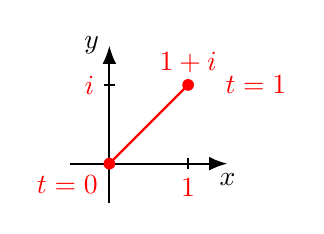
\begin{tikzpicture}[
    >=Latex, % Set default arrow tip style
    dot/.style={fill=red, circle, inner sep=1.5pt}, % Style for red points
    labelstyle/.style={red}, % Style for red labels
    tick/.style={thick} % Style for tick marks
]

    % Axes (adjust limits as needed)
    \draw[->, thick] (-0.5, 0) -- (1.5, 0) node[below] {$x$}; % x-axis label optional
    \draw[->, thick] (0, -0.5) -- (0, 1.5) node[left] {$y$}; % y-axis label optional

    % Define points
    \coordinate (start) at (0, 0); % t=0 at origin
    \coordinate (end) at (1, 1);   % t=1 at 1+i

    % Draw the red line segment
    \draw[red, thick] (start) -- (end);

    % Draw the points
    \node[dot] at (start) {};
    \node[dot] at (end) {};

    % Add Ticks
    \draw[tick] (1, -2pt) -- (1, 2pt); % Tick at x=1
    \draw[tick] (-2pt, 1) -- (2pt, 1); % Tick at y=1

    % Add Labels
    \node[labelstyle, below left=1pt of start] {$t=0$};
    \node[labelstyle, above=1pt of end] {$1+i$};
    \node[labelstyle, right=10pt of end] {$t=1$};
    \node[labelstyle, below=2pt] at (1, 0) {$1$}; % Label for x-axis tick
    \node[labelstyle, left=2pt] at (0, 1) {$i$}; % Label for y-axis tick

\end{tikzpicture}
\end{document}